\chapter{System Overview}

\begin{figure}[t]
  \centering
  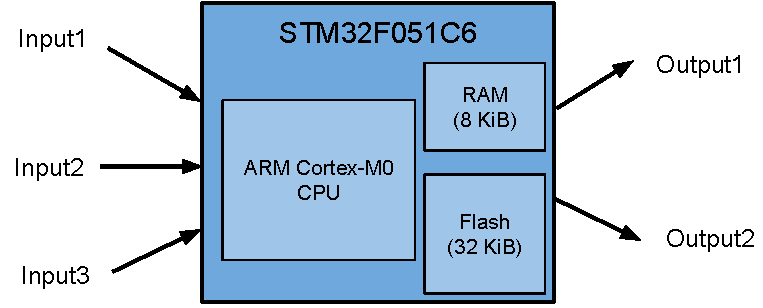
\includegraphics[width=\textwidth]{./week1/programmers_model_v0.pdf}
  \caption{The most simplified view of the internals of the STM32F051}
  \label{fig:prog_mod_v0}
\end{figure}

\section{What is a Microcontroller?}
The microcontroller can be understood by comparing it to something you are already very familiar with: the computer. Both a microcontroller and a computer can be modeled as a black box which takes in data and instructions, performs processing, and provides output.
In order to do this, a micro has some of the same internals as a computer, shown graphically in \autoref{fig:prog_mod_v0} and discussed now:
\begin{itemize}
  \item CPU: The section of the microcontroller which does the processing. It executes instructions which allows it to do arithmetic and logic operations, amongst other forms of operations.
  \item  Volatile memory (RAM:) This is general purpose memory. It can be used for storing whatever you want to store in it. Typically it stores variables which are created or changed during the course of execution of a program.
  \item Non-volatile memory (Flash): This non-volatile memory is used to store any date which must not be lost when the power to the micro is removed. Typically this would include the program code and any constants or initial values of data.
  \item Ports: Interfaces for data to move in and out of the micro. This allow it to communicate with the outside world. 
\end{itemize} 
These resources are typically orders of magnitude smaller or a micro than on a conventional computer. A micro makes up for this lack of resources with a small size, low power and low cost. A comparison of the characteristics can be seen in \autoref{table:specs_comp}.
A computer is typically defined as a multi-purpose, flexible unit able to do computation. A microcontroller on the other hand typically is hard-coded to do one specific job.\\

\begin{table}
\begin{tabu}{ >{\textbf}c | c  c  c  c  c  c }
  & \textbf{CPU} & \textbf{RAM} & \textbf{Non-volatile} & \textbf{Power} & \textbf{Size/Mass} & \textbf{Cost} \\
  \hline
  \textbf{Computer} & Dual, 3 GHz & 4 GiB & 500 GB & 100 W & Large & R 3000 \\
  \textbf{Micro} & 48 MHz & 8 KiB & 32 KiB & 50 mW & Small & R 15 \\
\end{tabu}
\caption{Comparison of specs of entry level computer to STM32F051C6.}
\label{table:specs_comp}
\end{table}

The terms micro\textit{controller} and micro\textit{processor} are different and should not be used interchangeably. A micro\textit{processor} is a chip which is able to perform computation, but requires external memory and peripherals to function. A micro\textit{controller} has the memory and peripherals built into it, allowing it to be fully independent. Furthermore, the interface in and out of a microprocessor is mainly just an address and data bus. In a microcontroller, these data and address busses are internal to the device. The interfaces in and out of a microcontroller are configurable to be a wide variety of communication standards. This self-contained nature and ability to deal with a wide variert of signals allows a microcontroller to (as the name suggest) be embedded in a larger system and perform control and monitoring functions.\\

The micro we will be using is the STM32F051C6. It is manufactured by ST Microelectronics, but has an ARM Cortex-M0 CPU. ARM designed the CPU (specified how the transistors connect together). ST then takes this CPU design, adds it to their design for all of the other bits of the micro (flash, RAM, ports and much much more) and then produces the chip.

\subsection{Development board block diagram}
The development board consists of modules which connect to the microcontroller. Most of these modules are optional in that they are not required for the microcontroller to run. We will develop code later in the course to interface with some of these modules. Those which are not optional are the voltage regulator and the debugger.
Following is a brief discussion of the purpose of each of the dev board modules (peripherals). You are not expected to know what many of these terms mean yet; this exists for you to refer back to later when you do encounter these perihperals. 

\begin{figure}
  \centering
  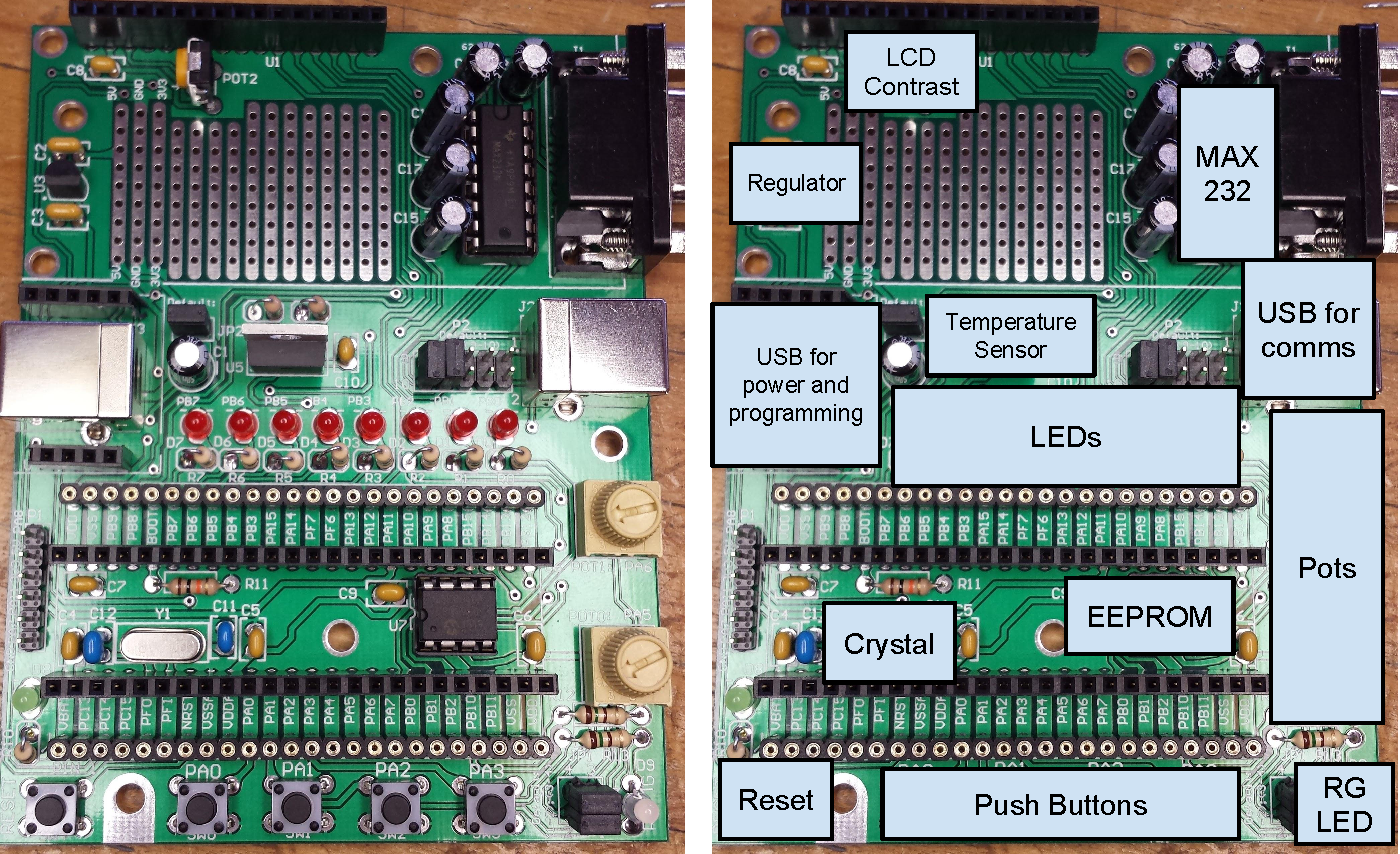
\includegraphics[width=\textwidth]{./week1/dev_board_unplugged.pdf}\\
  \vspace{3mm}
  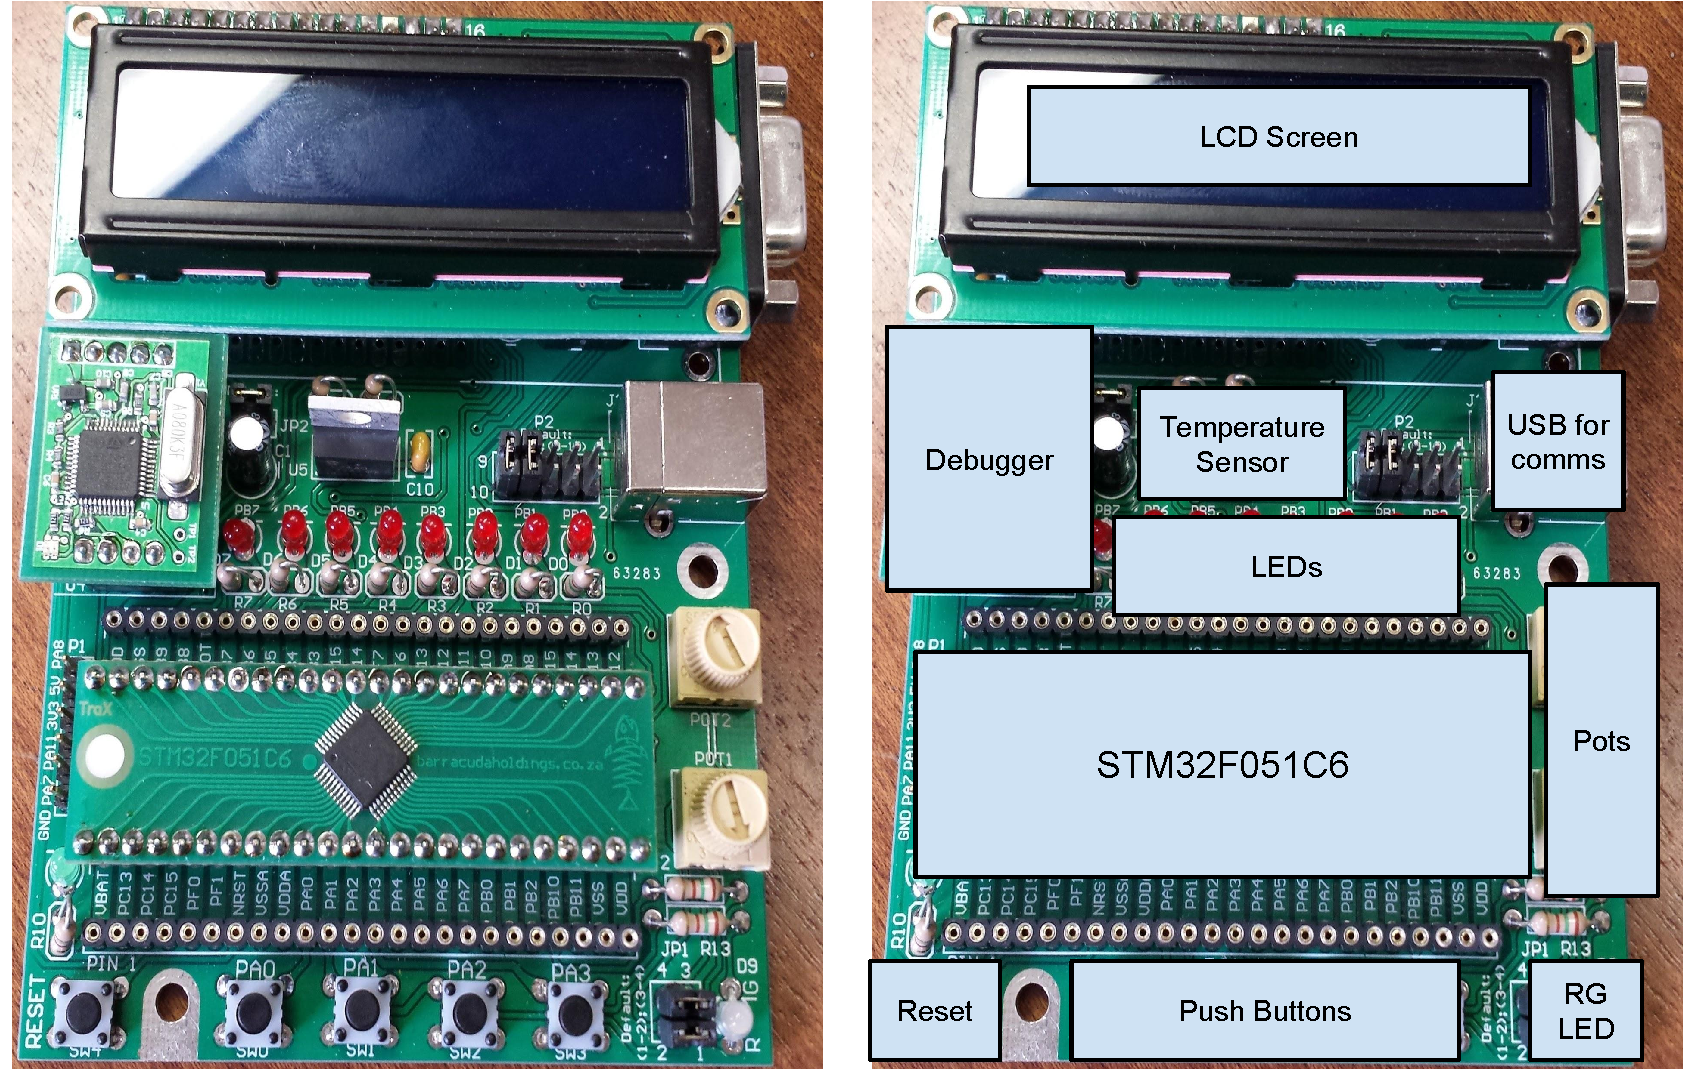
\includegraphics[width=\textwidth]{./week1/dev_board_plugged_in.pdf}
  \caption{Modules on the dev board as seen when top boards unplugged or plugged in.}
\end{figure}

\begin{itemize}
  \item STM32F051C6: This is the target microcontroller. It is connected to everything else on the board and it is where the code which we develop will execute. 
  \item Debugger: this is essentially another microcontroller running special code on it which allows it to be able to pass information between a computer and the target microcontroller. The interface to the computer is a USB connection, and the interface to the target is a protocol called Serial Wire Debug (SWD) which is similar to JTAG. The specific type of debugger which we have is a ST-Link.
  \item Regulator: A MCP1702-33/T0 chip. This converts the 5 V provided by the USB port into 3.3 V suitable for running most of the circuitry on the board. 
  \item LEDs: One byte of LEDs, active high connected to the lower byte of port B.
  \item Push buttons: Active low push buttons connected to the lower nibble of port A.
  \item Pots: 2 x 10K (or there abouts) potentiometers connected to PA5 and PA6.
  \item LCD Screen: A 16x2 screen connected to the micro in 4-bit mode. Used to display text.
  \item LCD contrast pot: The output of this potentiometer connects to the contrast pin of the LCD screen, hence allowing contrast adjustment.
  \item MAX232: This chips translates between TTL or CMOST logic level UART traffic and bi-polar higher voltage RS-232 traffic. Used for industrial communications links.
  \item USB for comms: The header allows intercepting of the UART traffic before it gets to the MAX232 and converting it to USB traffic through a small board which plugs into that header. When this facility is not being used, the jumpers on the header should be placed to allow the UART traffic to make its way to the MAX232.
  \item Temperature sensor: A TC74-A0 $I^2C$ temperature sensor.
  \item Crystal: 8 MHz quartz oscillator with 10 pF caps for removing high frequency harmonics. 
  \item EEPROM: A 25LC640A 64Kb Electronically Erasable and Programmable Read Only Memory (EEPROM) chip which communicates over SPI.
  \item RG LED: Common cathode Red/Green LED.
\end{itemize}


The full circuit schematic for the board follows. 
For now, we will forget about all of the other modules on the dev board and consider our system to be a computer talking to a debugger talking to a target micro, as shown in \autoref{fig:debugger_to_micro}. 
This is the most basic system which must be understood to allow us to load code onto the target microcontroller.

\begin{figure}[t]
  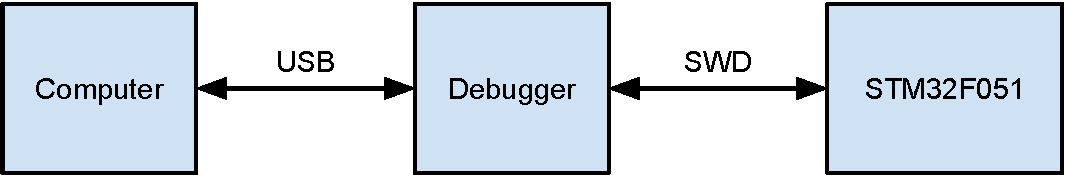
\includegraphics[width=\textwidth]{./week1/debugger_to_micro.pdf}
  \caption{Highly simpified diagram showing how micro and computer communicate}
  \label{fig:debugger_to_micro}
\end{figure}

\afterpage{
  \begin{landscape}
  %\begin{figure}
    \centering
    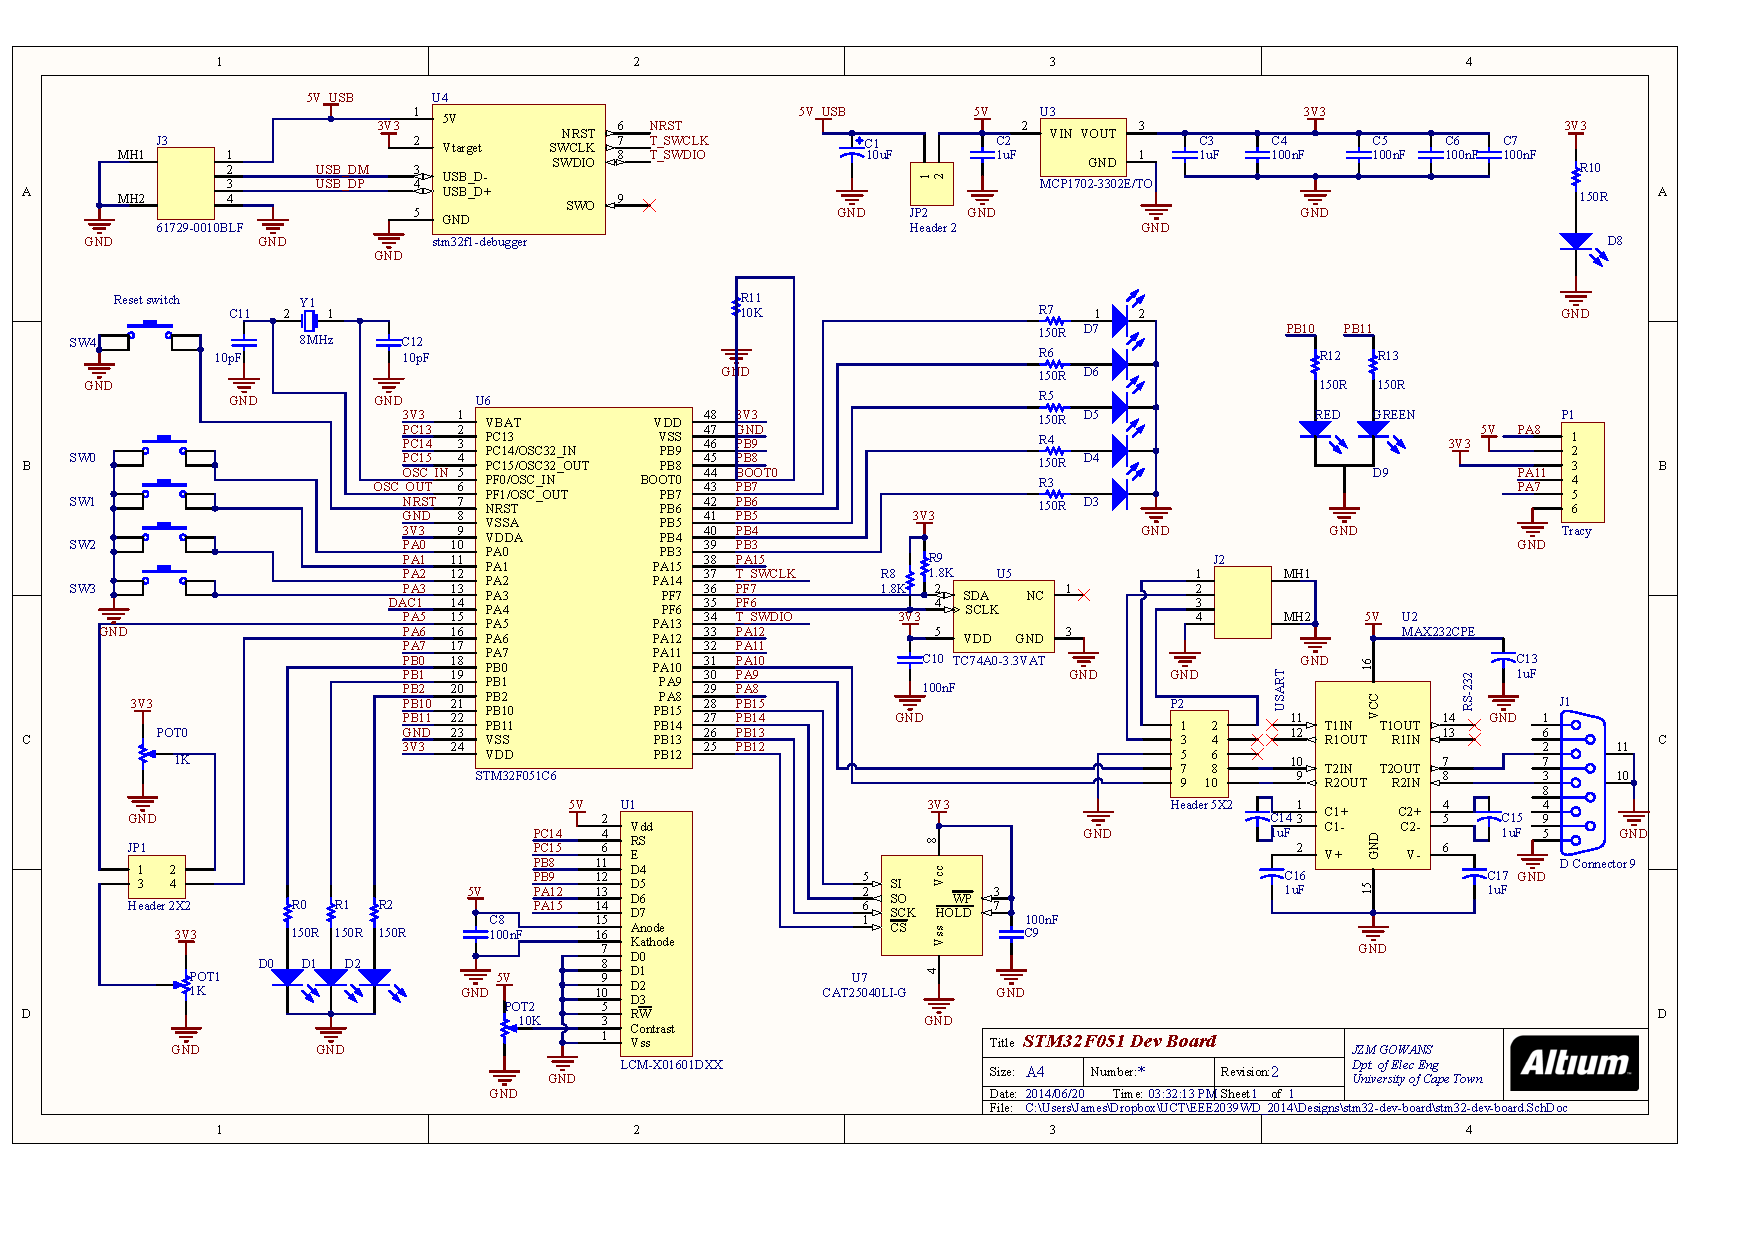
\includepdf[pages={1}, angle=90]{./week1/circuit_sch.pdf}
 % \end{figure}
 \end{landscape}
} 

%\subsection{A Short History of ARM}
%Acorn

%\chapter{Perihperals}
%Ports are typically controlled by a block of memory called perihperals. Unlike RAM which is general purpose, each register in the perihperals memory block has a specific, well defined purpose. Typically the purpose of these perihperal registes are for configuring the microcontroller to behave in a certain way or communicate with the outside world.
%These CPU registers are different to the peripheral registers mentioned earlier for the reasons that they are located inside the CPU rather than in the address space and also they are mostly general purpose: they can hold any data required in the execution of a program. 

